% !TEX root = ../ClassicThesis_DEIB.tex

\chapter{Grape hardware and software Architecure} \label{chap:grapeSoftwareArchitecture}

In this chapter we are going to describe in a detailed way the architecture of the robotic platform we used to implement the system to fulfill the requirements described in Section \ref{sec:grapeProjectDescription}. First, in Section \ref{sec:grapeHwArch}, we give an overview of the hardware components, from the robot base to all the actuators/sensors present on board. In Section \ref{sec:grapeSwArch}, we analyze the software architecture of the system, explaining what the main modules are, and the relationships between them.

\section{GRAPE hardware architecture}\label{sec:grapeHwArch}

\subsection{Robotic Base}
The choice of the robotic base is, of course, a crucial point in the development of our system, for two reasons:
\begin{itemize}
	\item without a well-functioning robotic base, no other objective can be achieved.
	\item the vineyard environment is particularly challenging in nature (this particular aspect is going to be well-justified in Chapter \ref{chap:localization}), thus a non-prudent choice could be very dangerous.
\end{itemize}
As anticipated in Section \ref{sec:odometry}, the choice fell on the \textbf{Husky} unmanned ground vehicle from Clearpath Robotics\footnote{\url{https://www.clearpathrobotics.com/husky-unmanned-ground-vehicle-robot/}},
(see Figure \ref{fig:husky}). There are several reasons for the adoption of this specific model:
\begin{itemize}
	\item it's a widely used platform (\textit{e.g.},: \cite{husky1}; \cite{husky2}; \cite{husky3}).
	\item it has a \textit{skid steering} kinematics that, as already seen in Section \ref{sec:odometry}, can be essentially reduced to a \textit{differential drive} kinematics, that is very simple.
	\item it's specifically designed for outdoor use, so robustness and ability to deal with unstructured terrain are problems addressed by its rugged construction and high-torque drivetrain.
	\item it offers a large payload capacity, to host the multitude of sensors, actuators and computational units we need.
	\item it's fully supported in \ac{ROS}, with open source drivers, configuration files and examples.
\end{itemize}

\begin{figure}
	\centering
	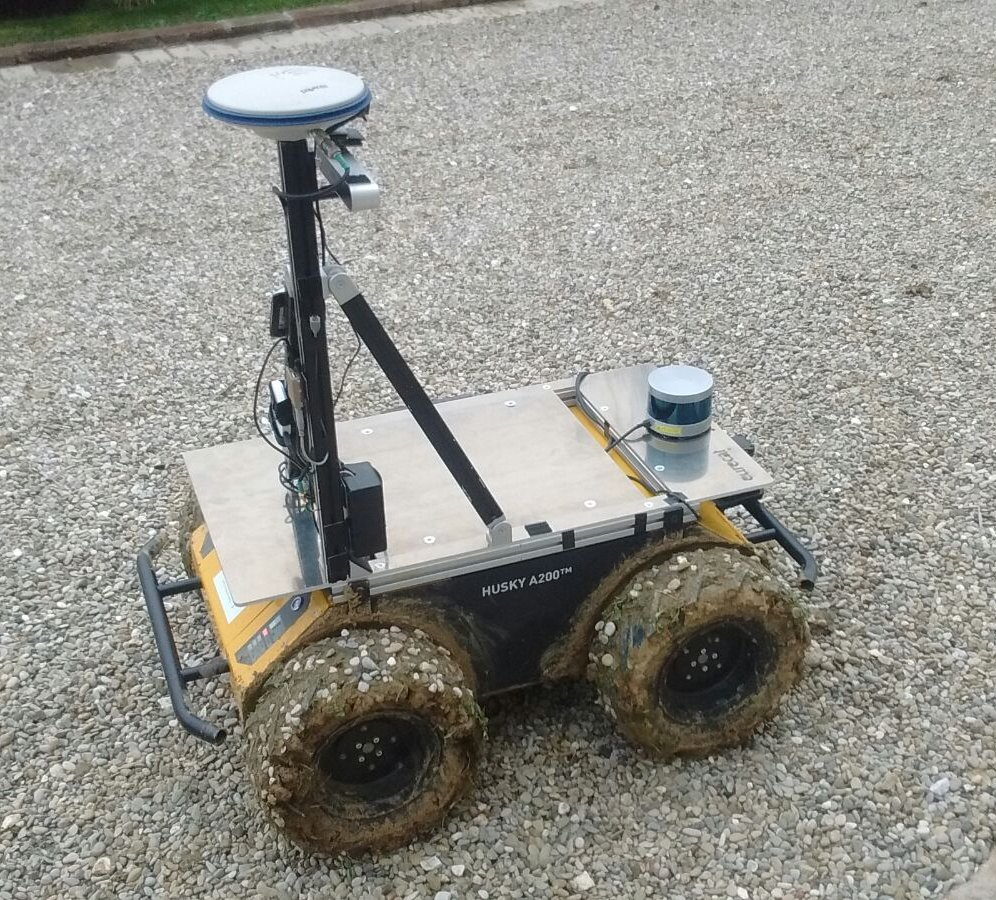
\includegraphics[width=0.5\textwidth]{Images/grape_sw_hw_architecture/ruoteFangose.jpeg}
	\caption{\textit{Husky platform after a navigation session in environment. You can easily note the amount of stones and mud stuck into the wheels.}}
	\label{fig:ruoteFangose}
\end{figure}

This choice turned out to be substantially good, since the \ac{ROS} drivers and configuration files were actually pretty easy to use and modify. The only major weakness identified in the Husky is related to its behavior on muddy ground, and is due to the wheels shape. After a few minutes of navigation in the mud, the unmanned ground vehicle tends to collect a significant amount of earth and stones in the wheels groves (see Figure \ref{fig:ruoteFangose}) and, consequentely, lose grip on the ground. This problem could be attenuated or solved by use of tracks instead of wheels.


\subsection{Robotic Arm}\label{subsec:kinovaArm}
By observing how pherormone dispensers must be deployed on the vine plant in Figure \ref{fig:dispensers} (in Figure \ref{fig:dispenserNostro}, you can see the dispenser shape that we actually used for \ac{GRAPE} project; in Figure \ref{fig:dispenserNostroDettaglio}, a close-up of our dispenser type), it's easy to understand that we require a very flexible robotic arm, with advanced movement capacity and capable of precise movement. Additional constraints also come from the limited space available on the Husky base, and from the limited power supply at disposal aboard. The choice fell on \textit{Jaco$^2$} arm from Kinova Robotics\footnote{\url{http://www.kinovarobotics.com/wp-content/uploads/2017/06/JACO\%C2\%B2-User-Guide-Asstive-Robotics-April-2017.pdf}}
(see Figure \ref{fig:kinovaArm}, Table \ref{tab:kinovaArmSpecs} for product specifications), for these reasons:
\begin{itemize}
	\item 6 DOF provide the required flexibility
	\item 3 fingers can be used for the dispensers deployment.
	\item while programmatic control is necessary for \ac{GRAPE} purpose, the joystick control makes it easy to perform quick tests and analyze the robot capabilities
	\item unlimited joints rotations.
	\item provided mechanical support for sensors mounting on top of the arm
	\item reduced weight and power consumption
	\item small overall dimensions
	\item \ac{ROS} open source drivers already provided by Kinova Robotics
\end{itemize}


\begin{table}[tb]
\footnotesize
\centering
\begin{tabularx}{0.6\textwidth}{lr}
\toprule
\tableheadline{l}{Parameter}  &
\tableheadline{r}{Value}  \\
\midrule
\tablefirstcol{l}{Degrees of Freedom}
& 6 \\
\midrule
\tablefirstcol{l}{Weight}
& 5.2 Kg \\
\midrule
\tablefirstcol{l}{Payload}
& 1.3 Kg \\
\midrule
\tablefirstcol{l}{Reach}
& 90 cm \\
\midrule
\tablefirstcol{l}{Maximum Linear arm speed}
& 20 $cm/s$ \\
\midrule
\tablefirstcol{l}{Power supply}
& $18\div29$ VDC \\
\midrule
\tablefirstcol{l}{Average Power}
& 25W \\
\midrule
\tablefirstcol{l}{Peak power}
& 100W \\
\midrule
\tablefirstcol{l}{Communication Protocol}
& RS485 \\
\midrule\tablefirstcol{l}{Material}
& Carbon fiber \\
\bottomrule
\end{tabularx}
\caption[Kinova Jaco$^2$ product specification]{Product specifications of Jaco$^2$ from Kinova Robotics.}
\label{tab:kinovaArmSpecs}
\end{table}


\begin{figure}
	\centering
	\subfloat[]{%
		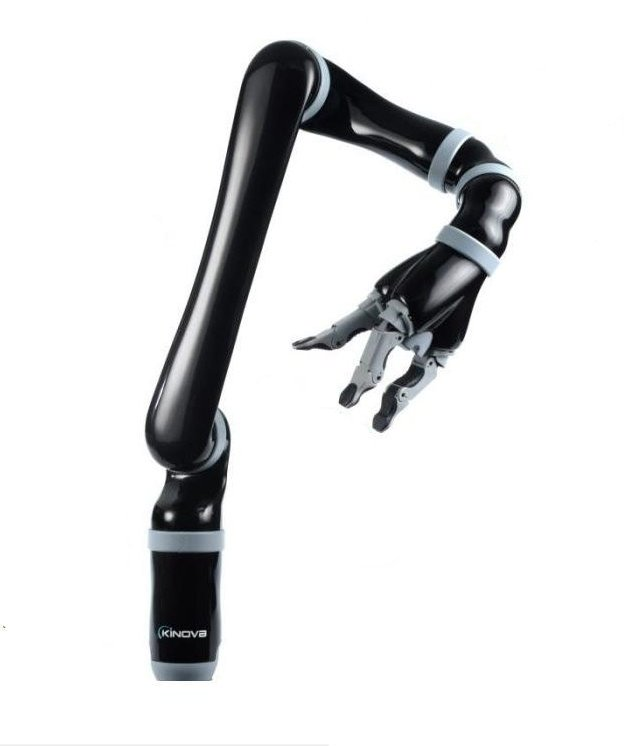
\includegraphics[width=0.5\textwidth]{Images/grape_sw_hw_architecture/kinova.jpg}
		\label{fig:kinovaArm}}
	\subfloat[]{%
		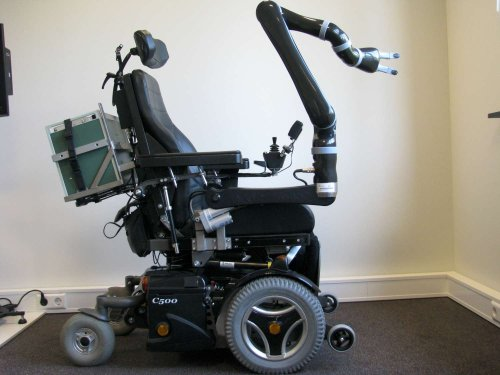
\includegraphics[width=0.4\textwidth]{Images/grape_sw_hw_architecture/kinovaCarrozzina.jpg}
		\label{fig:kinovaCarrozzina}}
	\caption{\textit{Robotic arm Jaco$^2$ with 3 fingers, from Kinova Robotics (\ref{fig:kinovaArm}) and the same arm mounted on a wheelchair \ref{fig:kinovaCarrozzina}}}
\end{figure}

 Some of the nice features of this device (weight, dimensions) actually derive from the original purpose of the arm, that is in the context of assistive devices for disabled people, to improve quality of life and independence of people on  electric powered wheelchairs (see Figure \ref{fig:kinovaCarrozzina}). But this fact also brought some unexpected weaknesses, that introduced a series of quite serious problems. The identified weaknesses are:
 \begin{itemize}
 	\item a very large imprecision in the movements piloted via programmatic control: this is probably due to joystick control seen as a "main control mode" since, as previously stated, the arm is born as an assistive device. This weakness was compensated partially modifying the open source drivers of the arm, and partially by the introduction of different control strategies. The magnitude of the error, measured as distance between the desired cartesian position of the end effector and the actual one, is $0\div3$ cm after the changes to the \ac{ROS} driver of the arm, and it was $0\div15$ before it.
 	\item buggy implementation of joints constraints, probably due to the same cause of the previous point. This created a major problem mostly because of the wiring used for the sensors (described in next sections) mounted on the arm, that kept entangling because of the unlimited joints rotation capability.
 \end{itemize}
 
After the analysis of the macro goals of \ac{GRAPE} project, it was decided to use the arm also as a support for other sensors for the dispenser deployment task: a \ac{LIDAR} and an RGB-D camera (see Figure \ref{fig:sensoriEndEffector}).
  
 \begin{figure}
	\centering
	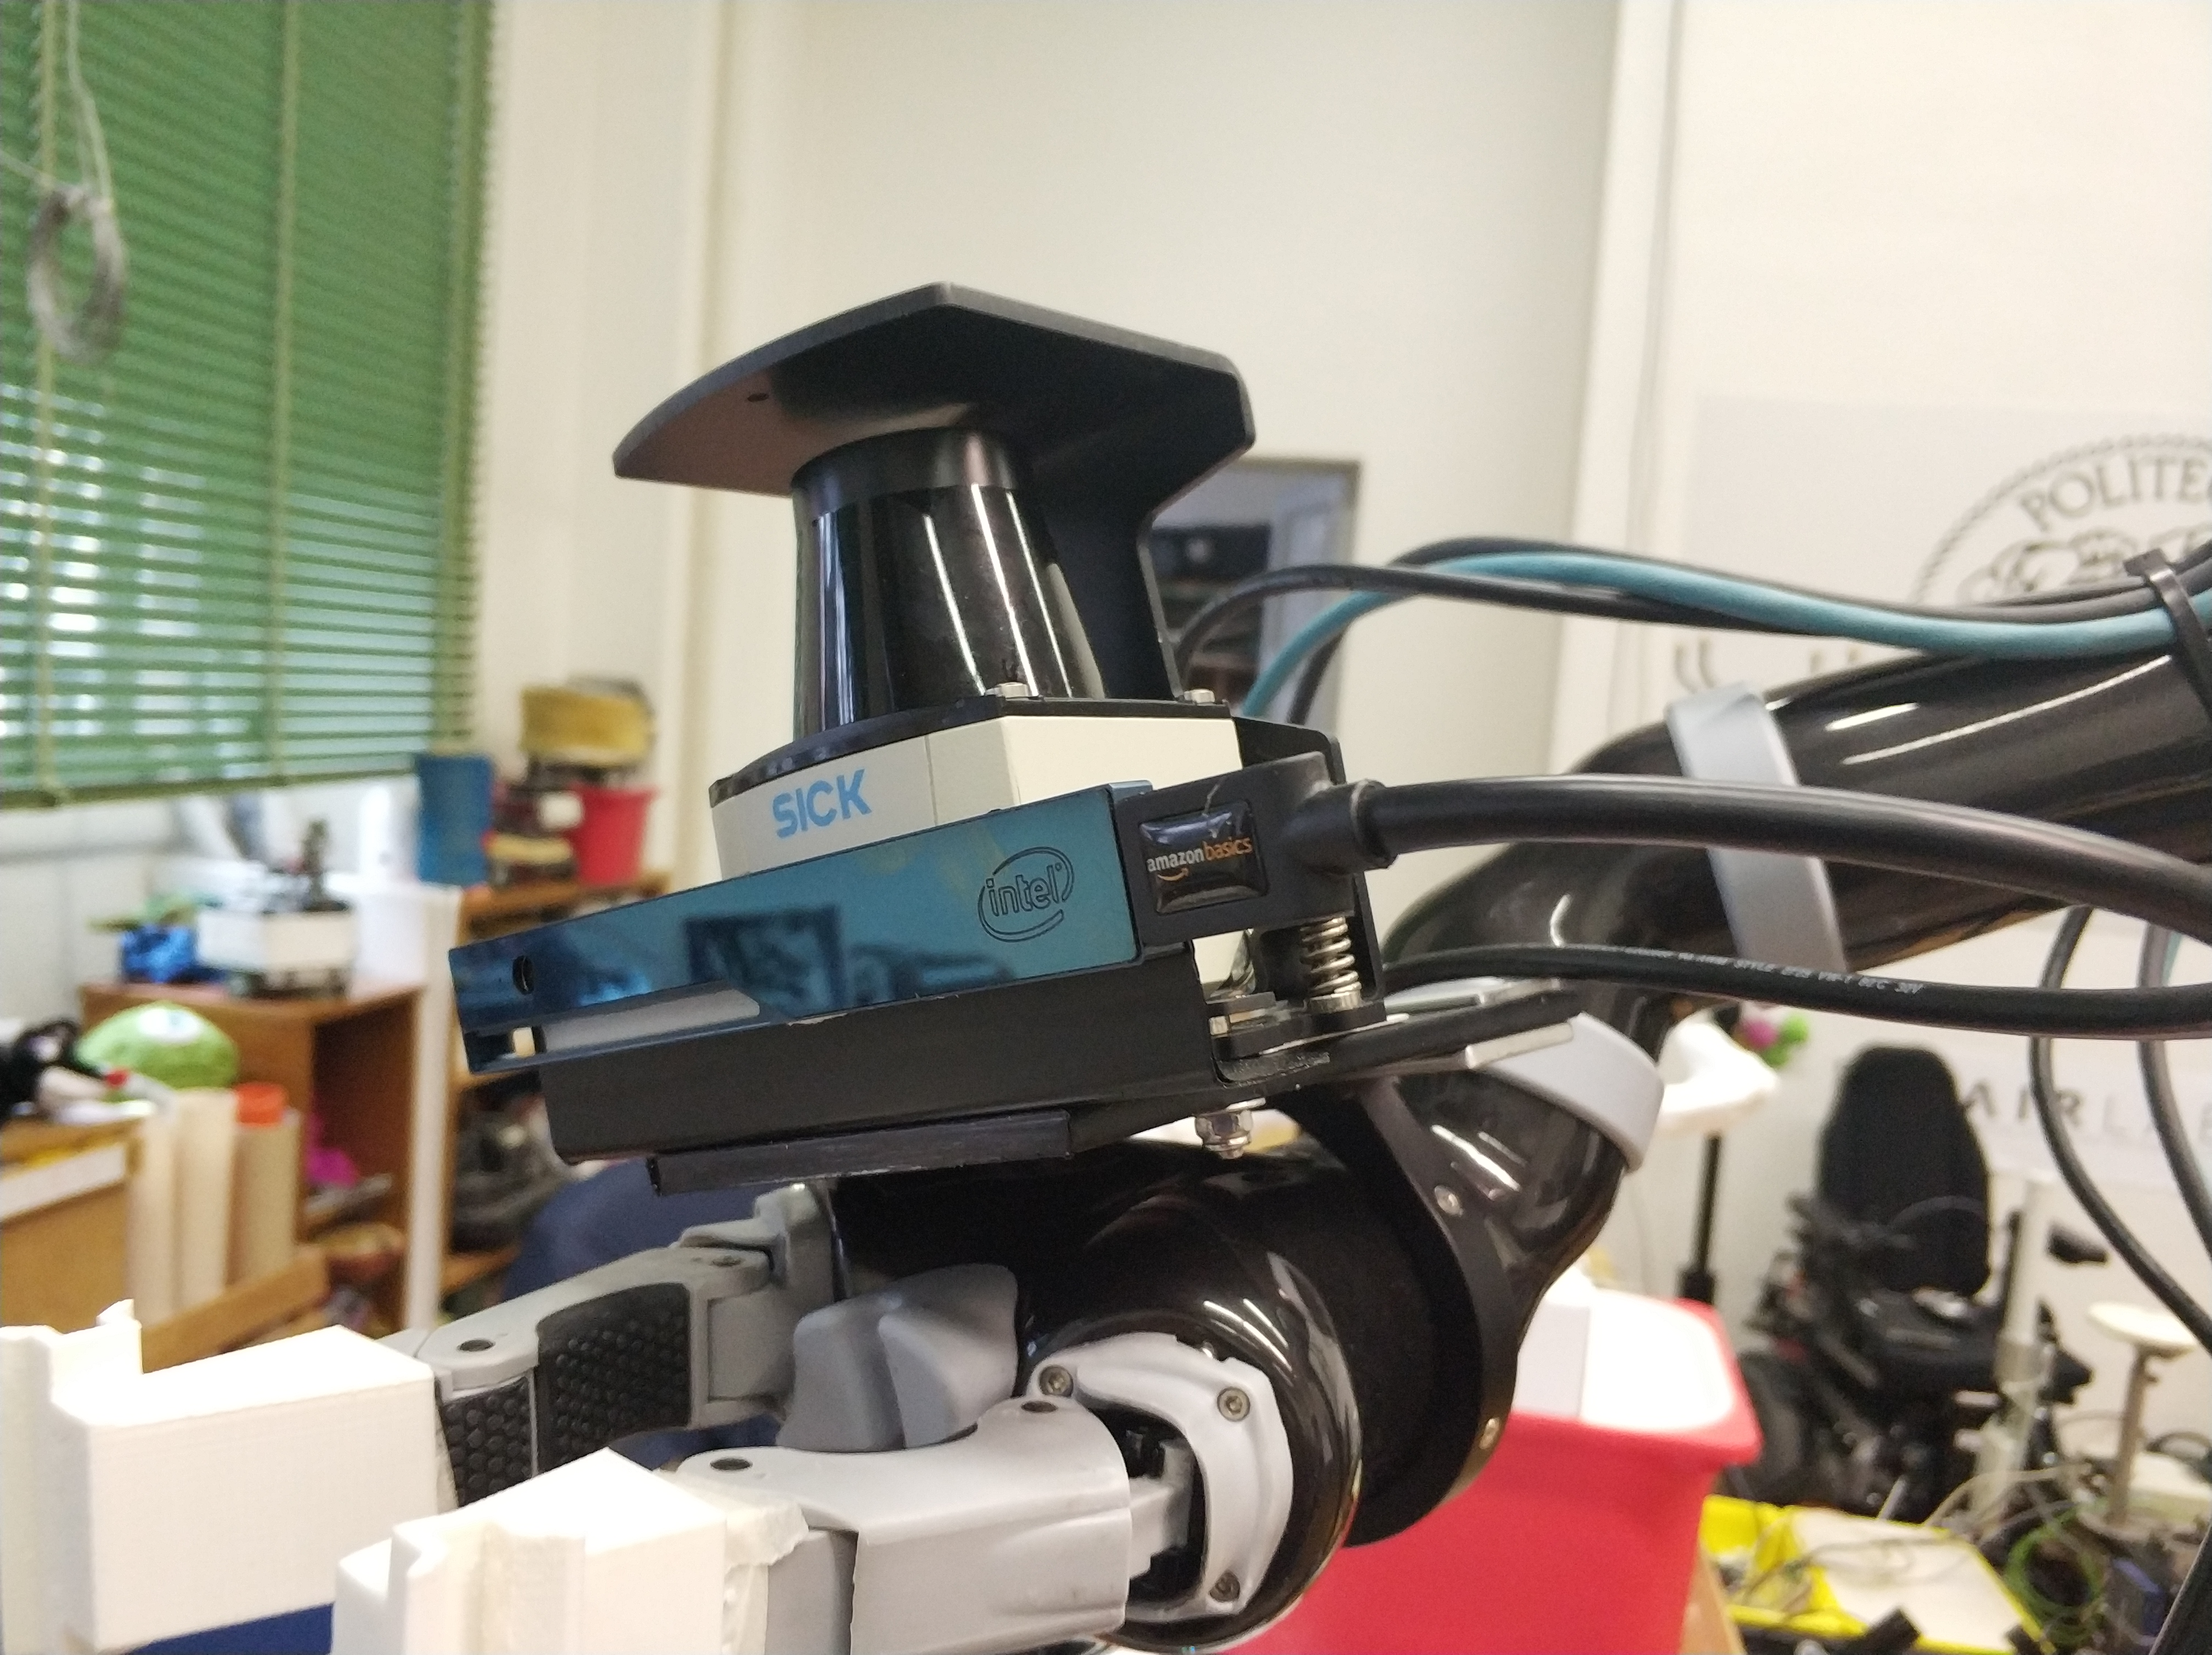
\includegraphics[width=0.5\textwidth]{Images/grape_sw_hw_architecture/sensoriEndEffector.jpg}
	\caption{\textit{The final configuration of the sensors (\ac{LIDAR} and RGB-D camera) mounted on top of the end effector.}}
	\label{fig:sensoriEndEffector}
\end{figure}

 \subsection{LIDARs}
 
 The final robotic system mounts three different \ac{LIDAR}s: two in front of the Husky for visualization and navigation purposes, and the other one mounted on a metal support on top of the arm end effector. The purpose of this last \ac{LIDAR} is explained in Chapter \ref{chap:kinovaArmChapter}; for now, all you need to know is that it's used in the procedure for the identification of the most suitable point for dispenser deployment. The \ac{LIDAR}s come from different producers, but they are quite similar being designed for outdoor use. The two used for navigation are \textbf{Velodyne VLP-16}\footnote{\url{http://velodynelidar.com/vlp-16-lite.html}}
 and \textbf{Hokuyo UTM-30LX-EW}\footnote{\url{https://www.hokuyo-aut.jp/search/single.php?serial=170}},
 the one on top of the arm is \textbf{SICK Tim561}\footnote{\url{https://www.sick.com/de/en/detection-and-ranging-solutions/2d-lidar-sensors/tim5xx/tim561-2050101/p/p369446}}.
 Main differences and similarities between these models are highlighted in Table \ref{tab:lidarComparison}


\begin{table}[tb]
\footnotesize
\centering
\begin{tabularx}{0.85\textwidth}{llll}
\toprule
\tableheadline{l}{}  &
\tableheadline{r}{VLP-16}  &
\tableheadline{r}{Tim561}  &
\tableheadline{r}{UTM-30LX-EW}  \\
\midrule
\tablefirstcol{l}{Number of Channels}
&16  &1 & 1\\
\midrule
\tablefirstcol{l}{Scan Angle}
&360°  & 270° & 270°\\
\midrule
\tablefirstcol{l}{Rotation rate}
&5Hz    & 15 Hz & 40Hz \\
&10Hz &  & \\
&20Hz &   & \\
\midrule
\tablefirstcol{l}{Angular Resolution}
& 0.1° & 0.33° & 025° \\
& 0.2°&\\
& 0.4°&\\
\midrule
\tablefirstcol{l}{Range}
&100m  & 10m & 30m\\
\midrule
\tablefirstcol{l}{Power Consumption}
&8W  & 4W& <8W\\
\midrule
\tablefirstcol{l}{Weight}
&590g  & 250g & 210g\\
\bottomrule
\end{tabularx}
\caption[Mounted \ac{LIDAR}s comparison]{Comparison of Husky on-board \ac{LIDAR}s }
\label{tab:lidarComparison}
\end{table}


\begin{figure}
	\centering
	\subfloat[]{%
		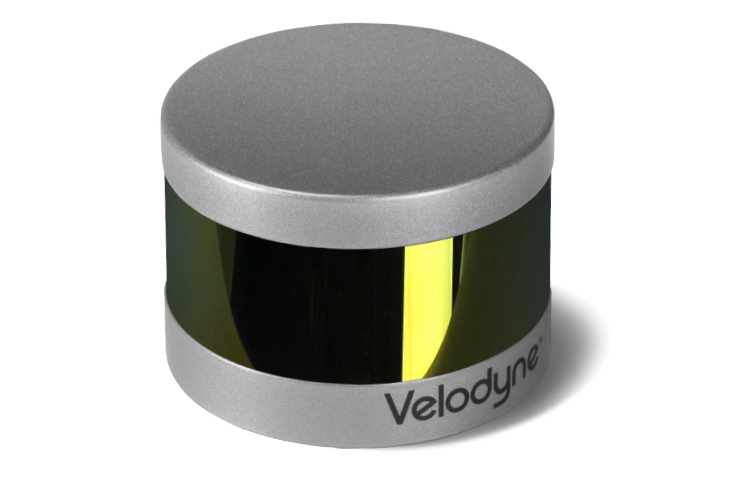
\includegraphics[width=0.3\textwidth]{Images/grape_sw_hw_architecture/velodynePuck.png}
		\label{fig:velodynePuckLite}}
	\subfloat[]{%
		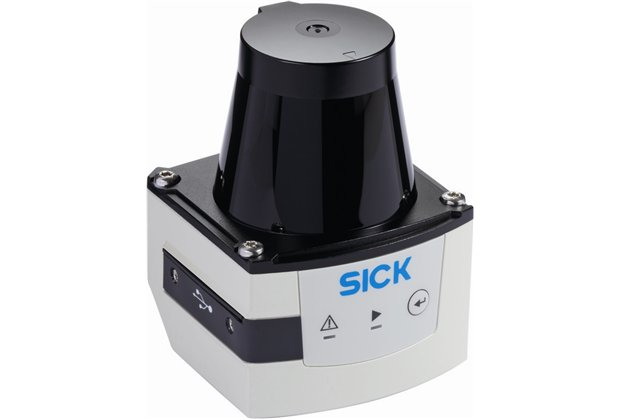
\includegraphics[width=0.35\textwidth]{Images/grape_sw_hw_architecture/sickTim561.jpg}
		\label{fig:sickTim561}}
%	\qquad
	\subfloat[]{%
		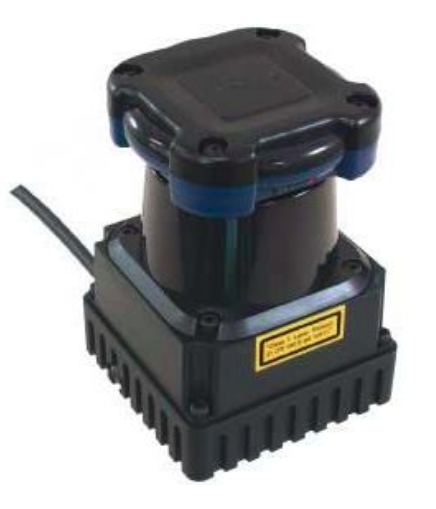
\includegraphics[width=0.25\textwidth]{Images/grape_sw_hw_architecture/hokuyo.png}
		\label{fig:hokuyo}}
	\caption{\textit{Three \ac{LIDAR}s mounted on our unmanned ground vehicle: Tim561 (\ref{fig:sickTim561}) from SICK, Puck Lite (\ref{fig:velodynePuckLite}) from Velodyne, UTM-30LX-EW (\ref{fig:hokuyo}) from Hokuyo.}}
\end{figure}

\subsection{RGB-D camera}
The other sensor mounted on top of the arm end effector is a \textbf{RealSense} RGB-D camera from Intel. This camera is able to sense the depth of the acquired images, by means of an active infrared stereo technology. The main usage of the camera is to provide images used for the feedback loop of the visual servo control of the Jaco$^2$ arm. Visual servoing is a technique which uses feedback information extracted from a vision sensor to control the motion of a robot \parencite{visualServo}, and it's used in this project to compensate the lack of precision in the arm motion operations (see Section \ref{subsec:kinovaArm}). This camera was also used in validation operations (validation of dispenser grasping, validation of dispenser deployment on the plant) and identification of exceptional cases (no dispensers left). 
\par The positive aspect of this camera model comes from its contained size and weight. We spotted only one significant weak point, that is a quite high minimum depth distance (20 cm), due to an intrinsic limit of the embedded depth technology. This problem created a few issues in dispenser application tasks, but they were easily bypassed.

\subsection{Tools for dispensers grasping}
Additional hardware was placed on the unmanned ground vehicle specifically for the accomplishment of the grasping of the dispenser, for two separate reasons:

\begin{itemize}
	\item the shape of the dispensers (see Figure \ref{fig:dispenserNostroDettaglio}) was not directly compatible with the grasping capability of the end effector of Jaco$^2$ arm (see the Jaco$^2$ fingers in Figure \ref{fig:kinovaArm}).
	\item the dispensers have to be stored on the Husky platform, in such a way to make them graspable.
\end{itemize}
We required custom hardware to accomplish these objectives so, given the prototype nature of the project, 3D stamped hardware was used.
For what concern the storage of the pheromone dispensers, the final version of the dispenser feeder was built out of two 3D-printed small towers (see Figure \ref{fig:dispenserFeeder}), with a sequence of very smooth aligned grooves, parallel to the horizontal plane, where the dispensers are slotted in. The smoothness of the grooves is the critical part of the design, indeed the previous versions of the towers, with sharper grooves, highlighted a difficulty of the grasping phase if the dispensers got caught on the feeder's corners.

\begin{figure}
	\centering
	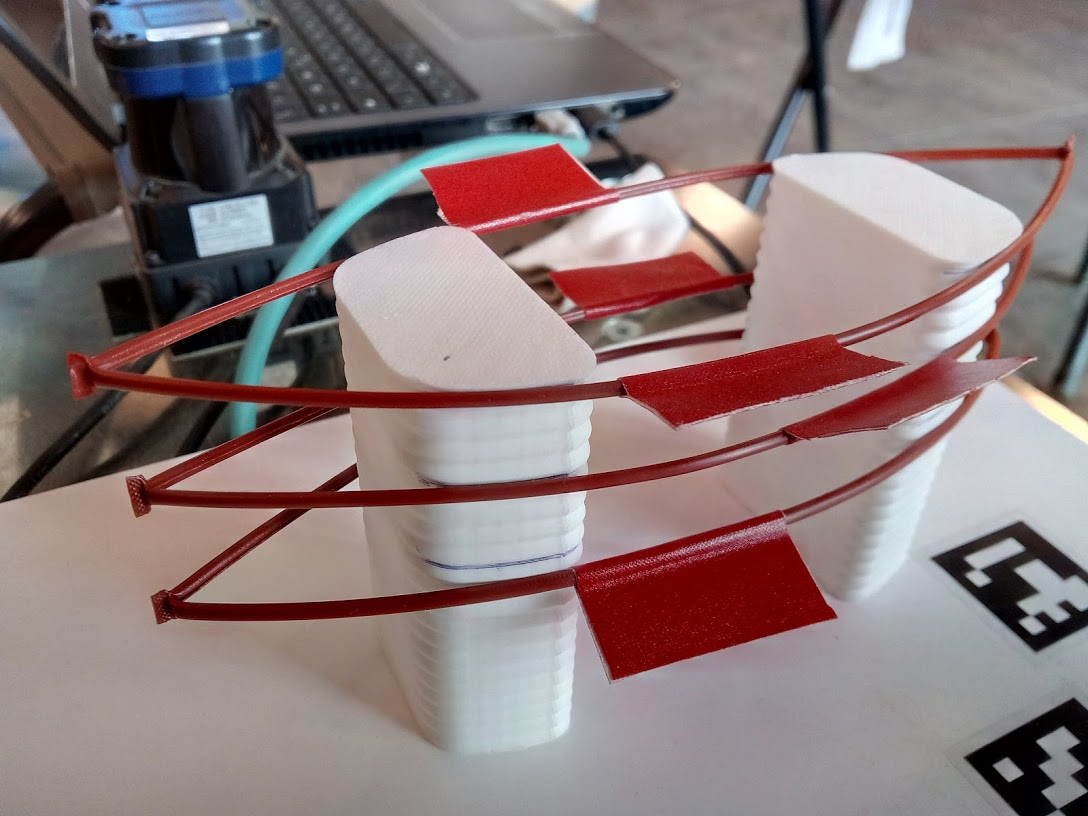
\includegraphics[width=0.6\textwidth]{Images/grape_sw_hw_architecture/feederConDispenser.jpg}
	\caption{\textit{The final version of the feeder, holding three dispensers.}}
	\label{fig:dispenserFeeder}
\end{figure}


The fingers of the robot are not all the same, because one of them act as a sort of "opposable thumb", that is useless in our application. So, two "nails" were printed to be applied to the two symmetric fingers, with a side dispenser-sized groove each, in order to grasp the dispenser by opening the two symmetric fingers.

\begin{figure}
	\centering
	\subfloat[]{%
		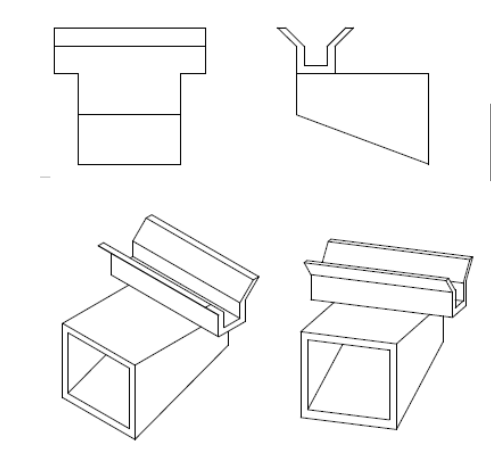
\includegraphics[width=0.3\textwidth]{Images/grape_sw_hw_architecture/unghieProspetto.png}
		\label{fig:unghieProspetto}}
	\subfloat[]{%
		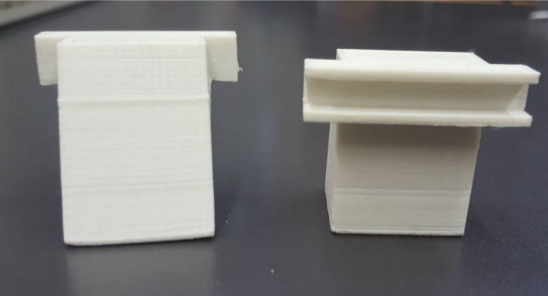
\includegraphics[width=0.4\textwidth]{Images/grape_sw_hw_architecture/unghieFoto.png}
		\label{fig:unghieFoto}}
	\caption{\textit{The final version of the 3D-printed nails (\ref{fig:unghieFoto}), and their 	perspective drawing (\ref{fig:unghieProspetto})}}
\end{figure}



\subsection{Other sensors}
The unmanned ground vehicle holds onboard a collection of other sensors, useful for the accomplishment of the established tasks. In this section we give a short overview of the few remaining ones:
\begin{description}
	\item[{IMU} sensor] Device including a magnetometer, accelerometer, gyroscope. These sensors were used in the odometry estimation system through sensor fusion algorithms (see Chapter \ref{chap:localization}).
	\item[GPS] Also this sensor data stream was included in the odometry estimation system.
	\item [Cameras] Additional camera mounted in a slightly lifted position with respect to the robot base; they are useful in case of teleoperation of the Husky or the robotic arm, and for visualization and monitoring purposes.
\end{description}

You can see the final sensor/actuators arrangement in Figure \ref{fig:disposizioneFinale}.
\begin{figure}
	\centering
	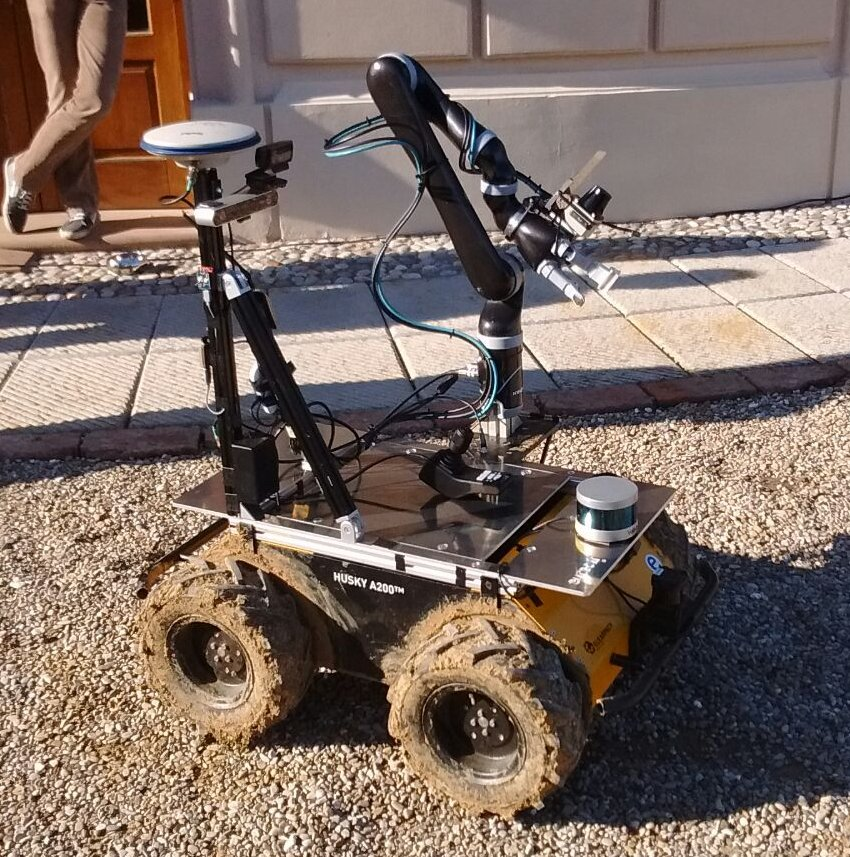
\includegraphics[width=0.6\textwidth]{Images/grape_sw_hw_architecture/disposizioneFinale.jpeg}
	\caption{\textit{The complete robotic platform, with sensors/actuators final arrangement.}}
	\label{fig:disposizioneFinale}
\end{figure}
 
\section{GRAPE software architecture}\label{sec:grapeSwArch}

Now that the hardware configuration is clear, we focus on the \textit{behavior} of the unmanned ground vehicle. We start by a description of the subproblems that we identified starting from the macro goals we talked about in Section \ref{sec:grapeProjectDescription}, and then move to the software architecture. \\

\subsection{Evaluation of vineyard navigation}
The problem of autonomous navigation of unmanned ground vehicles is a very well-known problem, studied at least from the nineties \parencite{storiaUGV}, because it's the first problem to deal with in almost all systems involving mobile robots. For this reason, and being our robotic system a prototype, the problem of vineyard navigation reduced to the following subproblems:
\begin{itemize}
	\item identification of a sensor fusion framework in \ac{ROS}, to provide an odometry estimate, and configuration of such a framework, with particular attention to which sensors fuse together.
	\item identification of a navigation framework in \ac{ROS}, to provide motion planning and speed control of the mobile base, and configuration of such a framework to fit our problem.
\end{itemize}
Even if these tasks could seem trivial, two major problems arose:
\begin{itemize}
	\item complex framework like these ones have tenths of parameter to tune, and the documentation is not always very precise.
	\item the \textit{off-the-shelf} navigation systems are usually born for indoor environments, that differ a lot from the very unstructured nature of the vineyards.
\end{itemize}

As hinted in Section \ref{sec:navigationStack} and \ref{subsec:robotLocalization}, our choices fell on \textbf{Move Base} package for the navigation, and \textbf{Robot Localization} as odometry system. More detail of the subproblems mentioned above are provided in Chapter \ref{chap:localization}.

\subsection{Evaluation of vineyard monitoring task}
For the vineyard monitoring task, as foreseen by the project proposal, we opted for a semi-autonomous monitoring: we provided the unmanned ground vehicle with a camera with video stream capability, that allows human users with competences in the domain of plants health to observe in person the live data streamed by the robot for assessment of crop condition. Human operators are also provided teleoperation interface for navigation and manipulation, for supervisioning and emergency handling function. This choice came from both the absence in the project proposal of precise objectives on this topic, and the complexity of feature extraction and evaluation in this context.

\subsection{Evaluation of dispenser application task}
 While the navigation task is a very common problem and \textit{off-the-shelf} solutions are easy to find, the dispenser application is a completely non-standard task, so we could only rely on libraries and packages for low-level subtasks and we had to design and implement the whole procedure from scratch. We divided the procedure in 3 subproblems:
 \begin{enumerate}
 	\item \textbf{Creation of a point cloud of the tree:} the robot is sitting still, with a vine on the same side of the Jaco$^2$ arm. When the procedure is triggered, the arm moves in order to produce a point cloud of the trees close to it, using the \ac{LIDAR} mounted onto it. 
 	\item \textbf{Deployment points identification:} once the point cloud has been produced, an algorithm based on \ac{PCL} trims the point cloud from the points that don't belong to the tree, process it, and outputs a sequence of 3D points $(x,y,z)$ corresponding to points on the tree suitable for the deployment of the dispenser, typically a protuberance of the tree, ordered from the best one to the worst one according to a suitable metric.
 	\item \textbf{Deployment of the dispenser:} the arm starts the dispenser deployment procedure, taking as input the sequence of points got in the previous step:
 	\begin{enumerate}
 		\item it grasps the dispenser (if any) from the dedicated support.
 		\item it applies the dispenser on the best feasible point from the input sequence.
 		\item it goes back to a retired position, to achieve better stability during the movement of unmanned ground vehicle.
 	\end{enumerate}
 	In Figure \ref{fig:deploymentOnMockup}, you can see an example of successful dispenser application, using the mockup plant. \textbf{NOTE:} the integration weeks were not all held in the same place (two of them in Garriguella (ES), and one in Casciana Terme (IT)), so we could observe that the vine trees shape is very different in the different locations (for example, the trees in Garriguella tend to have small almost vertical branches on the top of the pruned tree, while the Italian ones had smaller protuberances with variable orientation). 
 	\par This factor makes our system much harder to validate, because it's even more difficult to identify useful features in the unstructured vineyard environment. Thus, we introduced a further deployment mode, to be used in case our deployment procedure on the plants turned out not versatile enough to be efficient on a new tree type. Since we wanted to bypass the problems due to different tree structures, in this mode we assume to have some appropriately shaped nails, expressly arranged around the vineyard for dispenser applications. As described in Chapter \ref{chap:kinovaArmChapter}, this deployment mode also requires the application of \textit{binary square fiducial markers} (see Figure \ref{fig:arucoMarkers}), so in this way our application pushes a bit more towards a vineyard that modifies in order to be more suitable to robotic applications.
 	\par The steps of this deployment mode are slightly different from the previous ones:
 	\begin{enumerate}
 		\item it grasps the dispenser (if any) from the dedicated support.
 		\item it applies the dispenser on the nail, regardless of the input sequence (which become useless).
 		\item it goes back to a retired position, to achieve better stability during the movement of unmanned ground vehicle.
 	\end{enumerate}
 \end{enumerate}

\begin{figure}
	\centering
	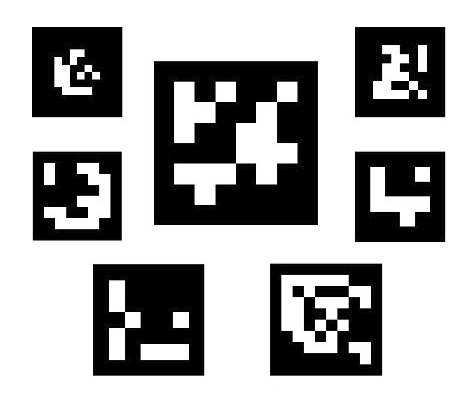
\includegraphics[width=0.4\textwidth]{Images/grape_sw_hw_architecture/arucoMarkers.png}
	\caption{\textit{Examples of visual binary fiducial markers (more specifically, ArUco markers) as the ones we used in visual servoing applications.}}
	\label{fig:arucoMarkers}
\end{figure}

\begin{figure}
	\centering
	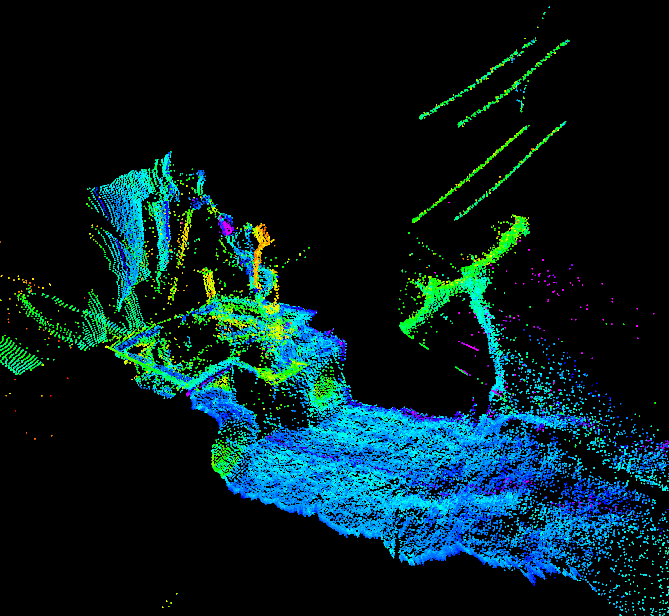
\includegraphics[width=0.6\textwidth]{Images/grape_sw_hw_architecture/scanPoints.png}
	\caption{\textit{Examples of laser scans collected in Casciana Terme during the integration week in January 2018, with the \ac{LIDAR} mounted on top of the end effector of the arm. You can recognize the vine plant, and part of the Husky base. The colors are only for visualization purpose.}}
	\label{fig:pointCloudScanned}
\end{figure}

\begin{figure}
	\centering
	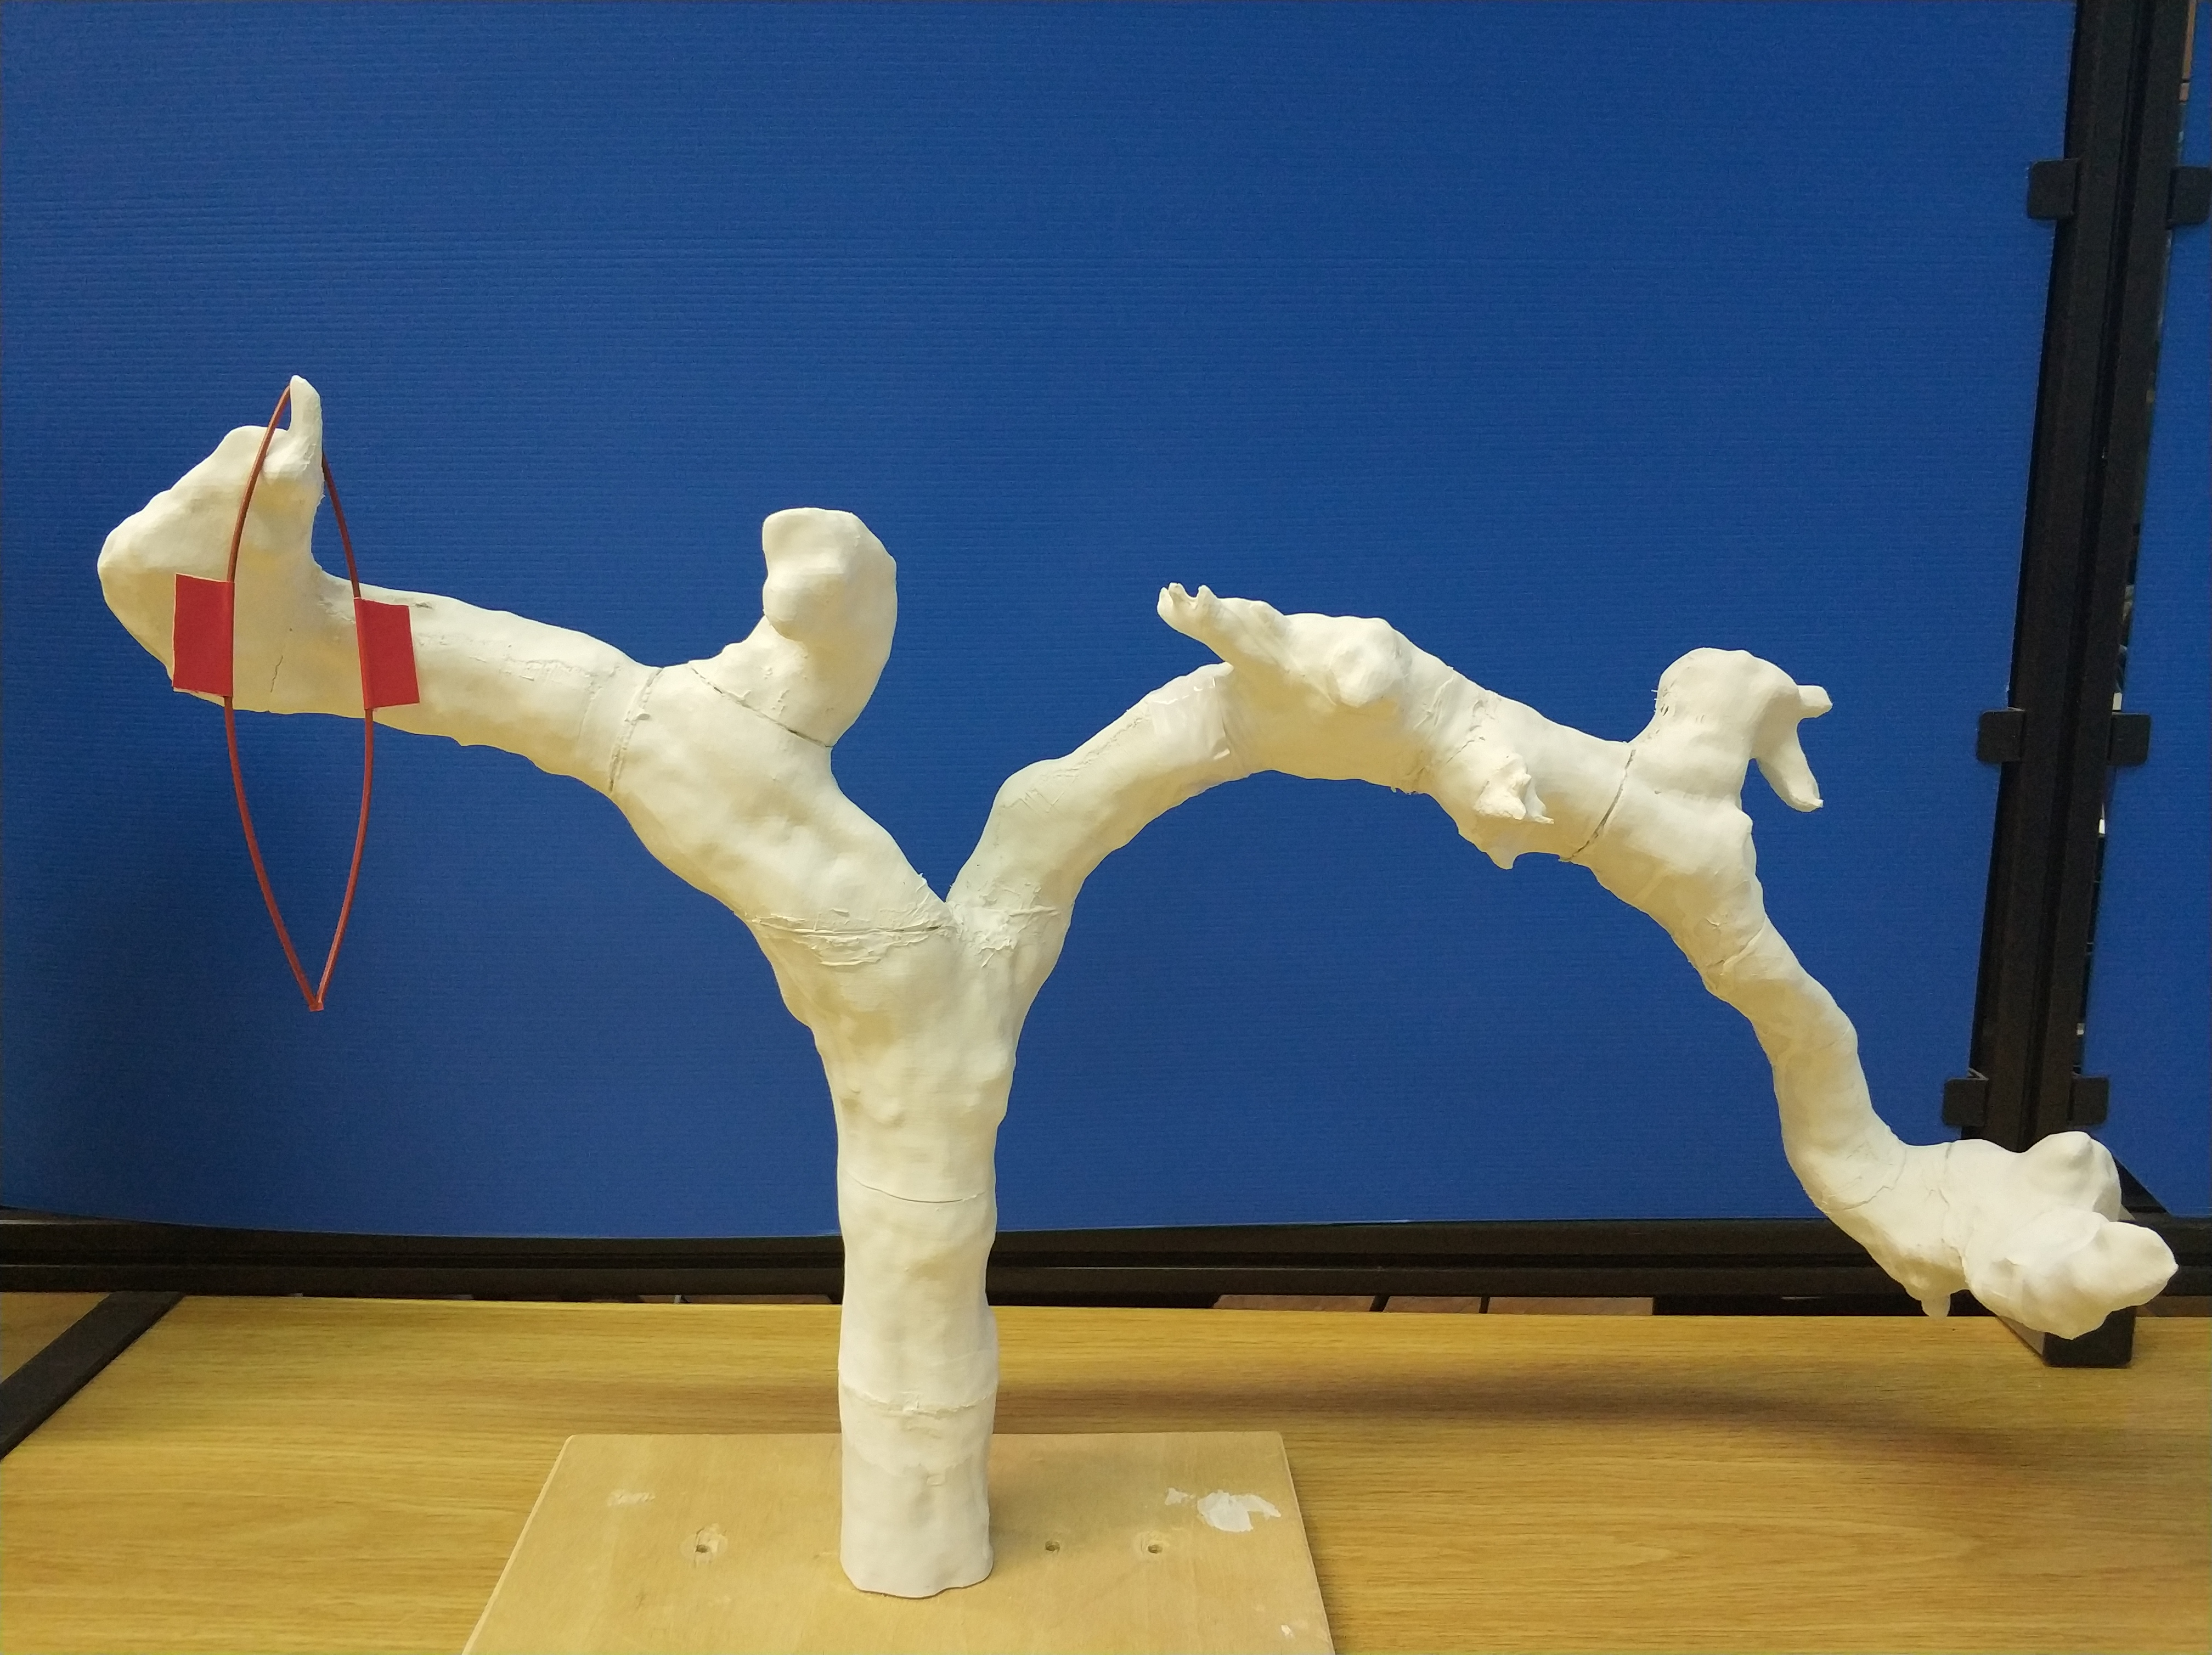
\includegraphics[width=0.6\textwidth]{Images/grape_sw_hw_architecture/deployOnMockup.jpg}
	\caption{\textit{Example of a dispenser application task, correctly executed on a mockup plant.}}
	\label{fig:deploymentOnMockup}
\end{figure}

All these procedures are quite long and complex, we wanted the user to have a high control on them, including the monitoring of intermediate results. For these reasons, these procedure are implemented as \ac{ROS} actions. 



\subsection{Details of the actions interfaces}

In this section we are giving a detailed description of the action interfaces, to better understand their scope and goals. Note that none of them includes a flag to check for correctness of execution, because we decided to use the internal status variable embedded in \ac{ROS} actions.

\subsubsection{Move Base action interface}
\begin{itemize}
	\item \textbf{Goal Message}:
		\begin{itemize}
			\item \textit{target\_pose}: the pose (position, orientation) we want our robot to reach
		\end{itemize} 
	\item  \textbf{Result Message}:
		\begin{itemize}
			\item \textit{base\_position}: the final pose (position, orientation) of the robot; in case of success, it should be very close to the specified \textit{target\_pose}
		\end{itemize} 
	\item  \textbf{Feedback Message}: \textit{n.a.}
\end{itemize}

\subsubsection{Scan motion action interface}
\begin{itemize}
	\item \textbf{Goal Message}: \textit{n.a.}
	\item  \textbf{Result Message}: \textit{n.a.}
	\item  \textbf{Feedback Message}: \textit{n.a.}
\end{itemize}
Note that even an empty \ac{ROS} action like this makes sense, because of the length (\textasciitilde30 seconds) of the procedure triggered by an action call.

\subsubsection{Point cloud processing action interface}
\begin{itemize}
	\item \textbf{Goal Message}: \textit{n.a.}
	\item  \textbf{Result Message}: 
		\begin{itemize}
			\item \textit{deployment\_pose}: contain an array ($x,y,z$) of possible deployment poses, identified from the plant point cloud; it's used as input to the dispenser deployment action server (see Table \ref{tab:processPointCloudAction})
		\end{itemize}
	\item  \textbf{Feedback Message}: \textit{n.a.}
\end{itemize}

\subsubsection{Dispenser deployment action interface}
\begin{itemize}
	\item \textbf{Goal Message}: 
		\begin{itemize}
			\item \textit{deployment\_poses}:  sequence of feasible deployment points, ordered from the best one to the worst one. These are the points output by \textit{Point cloud processing action}
			\item \textit{deploy\_mode}: an integer, used to select the technique to be used for the dispenser deployment; in fact, three different mode has been developed, in order to fit the different condition that the unmanned ground vehicle could face. In short, the modes available for selection are:
			\begin{itemize}
				\item Closed loop control, deployment target is an expressly placed nail, hammered into a pole.
				\item Closed loop control, deployment target is a protuberance of the vine tree.
				\item Open loop control, deployment target is a protuberance of the vine tree.
			\end{itemize}
			Details about the deployment mode are given in Chapter \ref{chap:kinovaArmChapter}.
		\end{itemize}

	\item  \textbf{Result Message}: \textit{n.a.}
	\item  \textbf{Feedback Message}: 
		\begin{itemize}
			\item \textit{ManipulationStatus status}: a message of proprietary type, which contains structures used to communicate the action caller the current execution state  (\textit{e.g.}, dispenser fallen, arm moving in front of the target point).
		\end{itemize}
\end{itemize}

\begin{table}[tb]
\footnotesize
\centering
\begin{tabularx}{0.85\textwidth}{ll}
\toprule
\toprule
\tablefirstcol{l}{\textbf{\texttt Goal Message}}
& \tt geometry\_msgs/PoseStamped target\_pose \\
\midrule
\tablefirstcol{l}{\textbf{\texttt Result Message}}
& \tt geometry\_msgs/PoseStamped base\_position \\
\midrule
\tablefirstcol{l}{\textbf{\texttt Feedback Message}}
& - - - \\
\bottomrule
\end{tabularx}
\caption[Move Base action specification]{Move Base action specification}
\label{tab:moveBaseAction}
\end{table}

 \begin{table}[tb]
\footnotesize
\centering
\begin{tabularx}{0.85\textwidth}{ll}
\toprule
\toprule
\tablefirstcol{l}{\textbf{\texttt Goal Message}}
& - - - \\
\midrule
\tablefirstcol{l}{\textbf{\texttt Result Message}}
& - - - \\
\midrule
\tablefirstcol{l}{\textbf{\texttt Feedback Message}}
& - - - \\
\bottomrule
\end{tabularx}
\caption[Scan motion action specification]{Scan motion action specification}
\label{tab:scanMotionAction}
\end{table}


 \begin{table}[tb]
\footnotesize
\centering
\begin{tabularx}{0.85\textwidth}{ll}
\toprule
\toprule
\tablefirstcol{l}{\textbf{\texttt Goal Message}}
& - - - \\
\midrule
\tablefirstcol{l}{\textbf{\texttt Result Message}}
& DeploymentPose[] deployment\_poses \\
\midrule
\tablefirstcol{l}{\textbf{\texttt Feedback Message}}
& int8 execution\_percent range [0,100] \\
\bottomrule
\end{tabularx}
\caption[Process point cloud action specification]{Process point cloud action specification}
\label{tab:processPointCloudAction}
\end{table}

 \begin{table}[tb]
\footnotesize
\centering
\begin{tabularx}{0.85\textwidth}{ll}
\hline
\toprule
\toprule
\tablefirstcol{l}{\textbf{\texttt Goal Message}}
& DeploymentPose[] deployment\_poses \\
& int32 deployMode \\
\midrule
\tablefirstcol{l}{\textbf{\texttt Result Message}}
& - - - \\
\midrule
\tablefirstcol{l}{\textbf{\texttt Feedback Message}}
& ManipulationStatus status \\
\bottomrule
\end{tabularx}
\caption[Dispenser Deployment action specification]{Dispenser Deployment action specification}
\label{tab:dispenserDeploymentAction}
\end{table}

\subsection{The supervisor}
Since all main operations in the project structure are implemented through action servers, a list of action clients must exists. For our implementation, we opted for a single software module that acts as an action client for all the actions mentioned above. We call this module \textit{Supervisor}, and its implementation uses behavior trees \parencite{behaviorTrees} as an overall model. The objective of the supervisor is to implement the global finite state automata of the system, where basically \textbf{nodes} are action servers or action clients. \\

\begin{tikzpicture}[->,>=stealth',shorten >=1pt,auto,node distance=2.1cm,
                    semithick, scale=0.6, every node/.style={scale=0.6},
                     palette1node/.style={shape=circle, draw=black,fill=palette1},
		  palette2node/.style={shape=circle, draw=black,fill=palette2},
		  palette3node/.style={shape=circle, draw=black,fill=palette3},
		  palette4node/.style={shape=circle, draw=black,fill=palette4},		  
  rednode/.style={shape=circle, draw=red, line width=2}]
   \label{fig:supervisorFSA}
  \tikzstyle{every state}=[fill=white,draw=black,text=black]

  \node[initial,state, fill=palette2] (A)         {$S_1$};
  \node[state, fill=palette4]                            (B) [above right = 0.7cm and 4.0cm of A] {$AS_1$};
  \node[state, fill=palette2]                            (C) [above left = 0.7cm and 4.0cm of B]  {$S_2$};
  \node[state, fill=palette3]                            (D) [above right = 0.7cm and 4.0cm of C] {$AS_2$};
  \node[state, fill=palette2]                            (E) [above left = 0.7cm and 4.0cm of D]  {$S_3$}; 
  \node[state, fill=palette2]                            (F) [above right = 0.7cm and 4.0cm of E] {$AS_3$};
  \node[state, fill=palette2]                            (G) [above left = 0.7cm and 4.0cm of F]  {$S_4$};
  \node[state, fill=palette3]                            (H) [above right = 0.7cm and 4.0cm of G] {$AS_4$};
  \node[state, fill=palette2]                            (I)   [above left = 0.7cm and 4.0cm of H] {$S_5$};
  
  \node (Z) [draw=palette5, fit= (A) (I), inner sep=3.5cm, 
            dashed, fill=blue!10, fill opacity=0.3, line width=0.7mm] {};
  \node [xshift=15ex,yshift=-1.5ex, palette5] at (Z.south) {Supervisor};
\path 
  (A) edge[sloped, anchor=center, below]    node{Move Base}(B)
  (B) edge[dotted, sloped, anchor=center, below]    node{Move Base}(C)
  (C) edge[sloped, anchor=center, below]    node{Scan Motion}(D)
  (D) edge[dotted, sloped, anchor=center, below]    node{Scan Motion}(E)
  (E) edge[sloped, anchor=center, below]    node{Point Extraction}(F)
  (F) edge[dotted, sloped, anchor=center, below]    node{Point Extraction}(G)
  (G) edge[sloped, anchor=center, below]    node{Deploy}(H)
  (H) edge[dotted, sloped, anchor=center, below]    node{Deploy}(I)
  (I)  edge[bend right,  sloped, anchor=left, below]    node{}(A)
  (C) edge[Maroon,bend right,  sloped, anchor=center, below]    node{}(A)
  (E) edge[Maroon,bend right,  sloped, anchor=center, below]    node{}(A)
  (G) edge[Maroon,bend right,  sloped, anchor=center, below]    node{}(A);  
  
	\node[palette2node,label=right:Eurecat, scale=2.0] (FD) at (10.5,14)   {};
	\node[palette3node,label=right:PoliMi, scale=2.0] (FD) at (10.5,13)   {};
	\node[palette4node,label=right:Already provided, scale=2.0] (FD) at (10.5,12)   {};
	\node[label=right:Error transition] at (10.5,11) {\textcolor{Maroon}{$\xrightarrow{\hspace{2.8em}}$}};
	\node[label=right:Action request] at (10.5,10) {$\xrightarrow{Action}$};
	\node[label=right:Action response] at (10.5,9) {$\xdashrightarrow{Action}$};
	\node[label=right:Normal transition] at (10.5,8) {$\xrightarrow{\hspace{2.8em}}$};	
  \end{tikzpicture}


As pointed out by Figure \ref{fig:supervisorFSA}, all action clients belong to the supervisor software module, and major tasks are implemented through action servers. In that graph we also specify the division of labor between the different teams:

\begin{itemize}
	\item Software modules assigned to \textbf{PoliMi}
		\begin{itemize}
			\item $AS_2$: Scan motion action server
			\item $AS_4$:	 Dispenser deployment action server
		\end{itemize}
	\item Software modules assigned to \textbf{Eurecat}
		\begin{itemize}
			\item $AS_2$: Point cloud processing action server
			\item $S_i$:	 Supervisor (\textit{i.e.}, all action clients and finite state automata implementation)
		\end{itemize}		
\end{itemize}

\subsection{Software modules treated in this thesis}

After this global overview of the hardware and software components of the \ac{GRAPE} project as a whole, we can finally specify which of the aforementioned topics has been directly treated in this thesis work. They are:
\begin{itemize}
	\item unmanned ground vehicle navigation system (see Chapter \ref{chap:localization})
	\item development of Scan motion action server (see Chapter \ref{chap:kinovaArmChapter})
	\item development of part of Dispenser deployment actions server (see Chapter \ref{chap:kinovaArmChapter})
\end{itemize}
